%-------------------------------------------------------------------------------
% This file provides a skeleton ATLAS note.
%-------------------------------------------------------------------------------
% Specify where ATLAS LaTeX style files can be found.
\newcommand*{\ATLASLATEXPATH}{latex/}
% Use this variant if the files are in a central location, e.g. $HOME/texmf.
% \newcommand*{\ATLASLATEXPATH}{}
%-------------------------------------------------------------------------------
\documentclass[PUB, UKenglish, texlive=2016]{\ATLASLATEXPATH atlasdoc}
% The language of the document must be set: usually UKenglish or USenglish.
% british and american also work!
% Commonly used options:
%  texlive=YYYY          Specify TeX Live version (2016 is default).
%  coverpage             Create ATLAS draft cover page for collaboration circulation.
%                        See atlas-draft-cover.tex for a list of variables that should be defined.
%  cernpreprint          Create front page for a CERN preprint.
%                        See atlas-preprint-cover.tex for a list of variables that should be defined.
%  NOTE                  The document is an ATLAS note (draft).
%  PAPER                 The document is an ATLAS paper (draft).
%  CONF                  The document is a CONF note (draft).
%  PUB                   The document is a PUB note (draft).
%  BOOK                  The document is of book form, like an LOI or TDR (draft)
%  txfonts=true|false    Use txfonts rather than the default newtx
%  paper=a4|letter       Set paper size to A4 (default) or letter.
---------------------------------------------------------------------
% Extra packages:
\usepackage[backend=biber,subcaption]{\ATLASLATEXPATH atlaspackage}
% Commonly used options:
%  biblatex=true|false   Use biblatex (default) or bibtex for the bibliography.
%  backend=bibtex        Use the bibtex backend rather than biber.
%  subfigure|subfig|subcaption  to use one of these packages for figures in figures.
%  minimal               Minimal set of packages.
%  default               Standard set of packages.
%  full                  Full set of packages.
%-------------------------------------------------------------------------------
\usepackage{authblk}
% Style file with biblatex options for ATLAS documents.
\usepackage{\ATLASLATEXPATH atlasbiblatex}

% Package for creating list of authors and contributors to the analysis.
\usepackage{\ATLASLATEXPATH atlascontribute}

% Useful macros
\usepackage{\ATLASLATEXPATH atlasphysics}
% See doc/atlas_physics.pdf for a list of the defined symbols.
% Default options are:
%   true:  journal, misc, particle, unit, xref
%   false: BSM, heppparticle, hepprocess, hion, jetetmiss, math, process, other, texmf
% See the package for details on the options.

% Files with references for use with biblatex.
% Note that biber gives an error if it finds empty bib files.
\addbibresource{mydocument.bib}
\addbibresource{bib/ATLAS.bib}
\addbibresource{bib/CMS.bib}
\addbibresource{bib/ConfNotes.bib}
\addbibresource{bib/PubNotes.bib}

% Paths for figures - do not forget the / at the end of the directory name.
\graphicspath{{logos/}{figures/}}

% Add you own definitions here (file mydocument-defs.sty).
\usepackage{mydocument-defs}

\usepackage{nicefrac}


%-------------------------------------------------------------------------------
% Generic document information
%-------------------------------------------------------------------------------

% Title, abstract and document 
\input{mydocument-metadata}
% Author and title for the PDF file
\hypersetup{pdftitle={ATLAS document},pdfauthor={The ATLAS Collaboration}}

%-------------------------------------------------------------------------------
% Content
%-------------------------------------------------------------------------------
\begin{document}

\maketitle

\tableofcontents

% List of contributors - print here or after the Bibliography.
%\PrintAtlasContribute{0.30}
%\clearpage

%-------------------------------------------------------------------------------
\section{Introduction}
\label{sec:intro}
%-------------------------------------------------------------------------------

Nowadays, Monte Carlo (MC) generators constitute the basic tool for particle-level perturbative predictions at the LHC. Whereas dedicated calculations exist at higher order for low-multiplicity particle production at parton level, Monte Carlo programs at next-to-leading order (\NLO) are highly automated for an extensive set of processes.

%-------------------------------------------------------------------------------
\section{Measurement of \ttbar observables}
\label{sec:analyses}
%-------------------------------------------------------------------------------

Event distributions generated by Herwig are compared against 7 TeV, 8 TeV and 13 TeV data measured by ATLAS. The distribution plots shown in Section \ref{sec:result} were produced with Rivet 2.4.0~\cite{Buckley:2010ar}. All the observables used for the tune are unfolded to particle level, and can be found in public Rivet analyses (with the exception of Analysis D, see below). More precisely, two sets of analyses are used for the studies presented in this document: a more general \textit{pre-study set} and a tentative \textit{tuning set}. The pre-study set comprises the following analyses:

\begin{itemize}

\item \textbf{Analysis A: Measurement of jet multiplicity and transverse momentum spectra in top events using full 7 TeV ATLAS dataset (ATLAS\_2014\_I1304688) \cite{Aad:2014iaa}}

This analysis measures the differential \ttbar production cross-section at a center-of-mass energy of 7 TeV in the lepton+jets channel. The distributions considered are the jet multiplicities with different jet transverse momentum thresholds, as well as the jet transverse momenta of up to the fifth leading jet. The jets and leptons are required to fulfill the $p_T > 25$ GeV and $|\eta| < 2.5$ kinematic requirements. The jets are clustered with the \antikt algorithm using a radius of $R=0.4$, and an overlap veto for $\Delta R(j, l) < 0.4$ and $\Delta R(j_1, j_2)<0.5$ is applied. Three or more jets are required to pass the vetoes, one of which has to be \btagged \footnote{Jets are \btagged using the MV1 algorithm, which combines results from track-based and secondary vertex reconstruction algorthms. (??need that??)}. (??rest of less usual cuts??)

\item \textbf{Analysis B: Measurement of jet shapes in top quark pair events at \sqs = 7 TeV (ATLAS\_2013\_I1243871) \cite{Aad:2013fba}}

Jet shapes originating from \ttbar events are measured in both the lepton+jets and dilepton channels. The differential and the integrated jet shapes from \bjets are compared to the ones initiated by light quarks. (??cuts??)

\item \textbf{Analysis C: Measurements of top-quark pair differential cross-sections in the lepton+jets channel in pp collisions at \sqs = 8 TeV (ATLAS\_2015\_I1404878) \cite{Aad:2015mbv}}

Measurements of the normalized differential cross-sections in \ttbar pair events were produced, as a function of the top quark, \ttbar system and other event-level kinematic observables.

\item \textbf{Analysis D: \ttbar+jets differential analysis and jet gap fractions at \sqs = 13 TeV in the dilepton channel (not yet published in Rivet)}


\end{itemize}

%-------------------------------------------------------------------------------
\section{Baseline setup}
\label{sec:setup}
%-------------------------------------------------------------------------------


A "best" baseline setup was chosen in accordance with the results from the pre-study analysis set, where the tunable generator parameters were left to their default values.

\subsection{MC generator}

For the main part of this study and wherever not explicitly precised, the MC events were generated by \HERWIG 7.0.3 in a local implementation. A comparison of the local setup with events generated in ATHENA can be found in \App{}. In principle, \HERWIG provides two different shower algorithms, namely an angular-ordered and a dipole shower. In parallel, it also features two matching schemes that are fully interchangeable: a subtractive and a multiplicative (\MCatNLO-like, respectively \POWHEG-like) scheme. All in all, the four combinations can be tried out, and the differences between the resulting distributions give an estimate of the systematic uncertainties associated with the missing higher-order terms (in \alphas and in uncancelled logarithmic contributions) stemming from the shower algorithms.

Although two separate shower implementations are provided in \HERWIG, only the default angular-ordered shower may be used for \ttbar production with the particular \HERWIG 7.0.3 generator version. Indeed, the decay of colored final-state particles is handled properly by the dipole shower only from \HERWIG 7.1.0 on. In contrast, both the subtractive and multiplicative matching schemes between the shower and the matrix elements can be enabled.

The generation of the matrix element amplitudes for \ttbar production at \NLO was handled by \GoSam ~\cite{Cullen:2011ac} via the Binoth-Les Houches interface (BLHA)\footnote{Also, for consistency the electroweak $G_{\mu}$-scheme was applied with $G_F=1.16637 \cdot 10^{-5}$ GeV$^{-2}$ for the Fermi constant. This choice does not affect the results (see \App)}. Additionally, there lies a residual theoretical freedom in the choice of the renormalization and factorization scales \muR and \muF. In the following, several meaningful choices were compared to data. Either a constant scale can be adopted, or one of the dynamical scales implemented in \HERWIG for \ttbar can be used. Two additional functional forms were tried out, following their definitions in ~\cite{Czakon:2016dgf}. All the nominal renormalization and factorization scale choices are summarized in Table \ref{setup:scalefuncs}. Here, \pT denotes the transverse momentum four-vector of the (anti-)top quark, and $m_T=\sqrt{m^2+p_T^2}$ its transverse mass.

\begin{table}[h]
\centering
\begin{tabular}{ l c c}

Functional form & Denomination & Implementation \\
\hline
$\muR=\muF=172.5$ \GeV & $m_t$ & \HERWIG \\ 
$\muR=\muF=\sqrt{(p_{T,t}+p_{T,\tbar})^2}$ & \TopPairMassScale & \HERWIG \\
$\muR=\muF=\sqrt{(1/2??)m_{T,t}^2+m_{T,\tbar}^2}$ & \TopMTScale & \HERWIG \\
$\muR=\muF=\sqrt{m_{T,t}+m_{T,\tbar}}$ & \TopLinSumMT & Custom  \\
$\muR=\muF=\frac{1}{2}\sqrt{m_{T,t} \cdot m_{T,\tbar}}$ & \HalfETScale & Custom \\

\end{tabular}
\caption{Several scale choices were tested: the ones available in \HERWIG that relate to top quark pair observables, and other possible choices which were implemented in a custom class. They will be referred to by name in the rest of this study.}
\label{setup:scalefuncs}
\end{table}

\subsection{Results}

\subsubsection{Scale dependence}

First, the dependence on the renormalization and factorization scale choice was asserted for the 7 TeV jet multiplicities and the 8 TeV kinematic observables. The \TopPairMassScale, \TopMTScale and the \ETScale scale were tested against each other, with various constant factors in front of their functional form. Figure \ref{setup:scaledeps} shows the results for a factor of \nicefrac{1}{2}. Note that here, the default \MCatNLO-like matching scheme was used. As can be seen, the jet activity is higher for both \TopPairMassScale and \TopMTScale. In particular, it is worth noting that predictions differ from the 5-jet bin on, i.e. already for the first emission. The choice of scale directly influences the value of \alphas at the first NLO branching, and the \HalfETScale scale agrees with data best. Also, and this is typical of the \MCatNLO-like matching scheme, the jet multiplicity is overestimated for the first emission, but underestimated in the high-multiplicity bins for the \HalfETScale scale, creating an "arc" in the jet multiplicity distributions. This effect is washed out for higher jet \pT cuts, though. 

Considering the kinematic variables at 8 TeV, the \HalfETScale scale is clearly preferred by both the \ttbar system' transverse momentum $p_T^{\ttbar}$ and the top-antitop azimuthal angle $\Delta \phi_{\ttbar}$ distributions. The tail in the high-mass region of the \ttbar system's invariant mass distribution rules the \TopPairMassScale out. Finally, the fiducial cross-section is consistently 10\% higher than experimental data, as can be seen in the $|y_{\ttbar}|$ distribution. Indeed, although the total cross-section is normalized to the computed NNLO+NNLL \ttbar production cross-section, the generated events surviving the analysis cuts are in excess. In Figure \ref{setup:scaledeps1factor}, the same functional forms are compared for kinematic variables, but with a prefactor of 1. In conclusion, the scale fitting all distributions best is the \HalfETScale scale. From now on, we assume this choice for the renormalization and factorization scales, except if explicitly said otherwise.

\begin{figure}
\centering
	\begin{subfigure}[b]{0.4\textwidth}
	\includegraphics[width=\textwidth]{setup/scaleDep/7TeV/d01-x01-y01.pdf}
	\end{subfigure} 
	~
	\begin{subfigure}[b]{0.4\textwidth}
	\includegraphics[width=\textwidth]{setup/scaleDep/7TeV/d01-x03-y01.pdf}
	\end{subfigure}
	
	\begin{subfigure}[b]{0.4\textwidth}
	\includegraphics[width=\textwidth]{setup/scaleDep/8TeV0.5/d01-x01-y01.pdf}
	\end{subfigure}
	~
	\begin{subfigure}[b]{0.4\textwidth}
	\includegraphics[width=\textwidth]{setup/scaleDep/8TeV0.5/d03-x01-y01.pdf}
	\end{subfigure}
	
	\begin{subfigure}[b]{0.4\textwidth}
	\includegraphics[width=\textwidth]{setup/scaleDep/8TeV0.5/d13-x01-y01.pdf}
	\end{subfigure}
	~
	\begin{subfigure}[b]{0.4\textwidth}
	\includegraphics[width=\textwidth]{setup/scaleDep/8TeV0.5/d05-x01-y01.pdf}
	\end{subfigure}
	\caption{Jet multiplicities at 7 TeV and kinematic observables at 8 TeV are compared for the three scales \TopPairMassScale, \TopMTScale and the \ETScale scale with a constant factor of \nicefrac{1}{2}. The current matching scheme is the subtractive one.}
	\label{setup:scaledeps}
\end{figure}

\begin{figure}
\centering
	\begin{subfigure}[b]{0.4\textwidth}
	\includegraphics[width=\textwidth]{setup/scaleDep/8TeV1.0/d01-x01-y01.pdf}
	\end{subfigure} 
	~
	\begin{subfigure}[b]{0.4\textwidth}
	\includegraphics[width=\textwidth]{setup/scaleDep/8TeV1.0/d03-x01-y01.pdf}
	\end{subfigure}
	
	\caption{The \ttbar system's invariant mass and transverse momentum distributions are plotted for the \TopPairMassScale, \TopMTScale and the \ETScale scale with a prefactor of 1.0. Both \TopMTScale and \ETScale scales behave comparably, but the agreement with data is still worse than the \HalfETScale scale.}
	\label{setup:scaledeps1factor}
\end{figure}

\subsubsection{Matching scheme}

As mentioned above, the angular-ordered shower can be matched to the NLO matrix element via two matching schemes, namely an \MCatNLO-like and a \POWHEG-like scheme. Still using the \HalfETScale choice as a functional form for the renormalization and factorization scales, Figure \ref{setup:matchdeps} compares both matching schemes at 7 TeV and 8 TeV.

The jet multiplicities at 7 TeV underline the disappearance of the \MCatNLO arc effect once going to the \POWHEG-like scheme, which flattens the distribution up to the $8^{\textrm{th}}$ jet. For higher jet \pT cuts, the jet activity is still too low.

\begin{figure}
\centering
	\begin{subfigure}[b]{0.4\textwidth}
	\includegraphics[width=\textwidth]{setup/matchScheme/7TeV/d01-x01-y01.pdf}
	\end{subfigure} 
	~
	\begin{subfigure}[b]{0.4\textwidth}
	\includegraphics[width=\textwidth]{setup/matchScheme/7TeV/d01-x03-y01.pdf}
	\end{subfigure}
	
	\begin{subfigure}[b]{0.4\textwidth}
	\includegraphics[width=\textwidth]{setup/matchScheme/8TeV/d01-x01-y01.pdf}
	\end{subfigure}
	~
	\begin{subfigure}[b]{0.4\textwidth}
	\includegraphics[width=\textwidth]{setup/matchScheme/8TeV/d03-x01-y01.pdf}
	\end{subfigure}
	
	\begin{subfigure}[b]{0.4\textwidth}
	\includegraphics[width=\textwidth]{setup/matchScheme/8TeV/d13-x01-y01.pdf}
	\end{subfigure}
	~
	\begin{subfigure}[b]{0.4\textwidth}
	\includegraphics[width=\textwidth]{setup/matchScheme/8TeV/d05-x01-y01.pdf}
	\end{subfigure}
	\caption{Jet multiplicities at 7 TeV and kinematic observables at 8 TeV are compared for the three scales \TopPairMassScale, \TopMTScale and the \ETScale scale with a constant factor of \nicefrac{1}{2}}
	\label{setup:matchdeps}
\end{figure}


%-------------------------------------------------------------------------------
\section{Toy parameters and results}
\label{sec:result}
%-------------------------------------------------------------------------------

Place your results here.

% All figures and tables should appear before the summary and conclusion.
% The package placeins provides the macro \FloatBarrier to achieve this.
% \FloatBarrier


%-------------------------------------------------------------------------------
\section{Conclusion}
\label{sec:conclusion}
%-------------------------------------------------------------------------------

Place your conclusion here.


%-------------------------------------------------------------------------------
% If you use biblatex and either biber or bibtex to process the bibliography
% just say \printbibliography here
\printbibliography
% If you want to use the traditional BibTeX you need to use the syntax below.
%\bibliographystyle{bib/bst/atlasBibStyleWithTitle}
%\bibliography{mydocument,bib/ATLAS,bib/CMS,bib/ConfNotes,bib/PubNotes}
%-------------------------------------------------------------------------------

%-------------------------------------------------------------------------------
% Print the list of contributors to the analysis
% The argument gives the fraction of the text width used for the names
%-------------------------------------------------------------------------------
\clearpage
The supporting notes for the analysis should also contain a list of contributors.
This information should usually be included in \texttt{mydocument-metadata.tex}.
The list should be printed either here or before the Table of Contents.
\PrintAtlasContribute{0.30}


%-------------------------------------------------------------------------------
\clearpage
\appendix
\part*{Appendices}
\addcontentsline{toc}{part}{Appendices}
%-------------------------------------------------------------------------------

In an ATLAS note, use the appendices to include all the technical details of your work
that are relevant for the ATLAS Collaboration only (e.g.\ dataset details, software release used).
This information should be printed after the Bibliography.

\end{document}
